\documentclass[12pt]{article}

\usepackage[utf8]{inputenc}
\usepackage{geometry, graphicx, booktabs, array, paralist, verbatim, subfig, amsfonts, amsmath, amssymb, fancyhdr, amsthm, polynom, setspace, enumitem, gensymb, xfrac, mathtools, titling, wasysym, sectsty, xcolor, epstopdf, appendix, natbib, lmodern, pagecolor, afterpage, lastpage, lipsum, tikz, wrapfig, indentfirst, floatflt, picins, csvsimple, pgfplotstable, colortbl, hyperref, refcount}
\usepackage[pages=some]{background}

\geometry{a4paper, lmargin=0.5in, rmargin=0.5in}
\pagestyle{fancy}
\fancyhf{}

\definecolor{wernergold}{RGB}{247, 155, 47}
\definecolor{wernerblue}{RGB}{27, 54, 93}
\definecolor{wernersky}{RGB}{141, 200, 232}
\definecolor{wernermedblue}{RGB}{123, 164, 219}

\renewcommand{\headrulewidth}{1.5pt}
\renewcommand{\footrulewidth}{1.5pt}

\lhead{David Cavanaugh}\chead{}\rhead{Math 8670: Advanced Statistical Machine Learning}
\lfoot{\textit{Predicting Wildfires}}\cfoot{\vspace{-10pt}\hyperref[sec:introduction]{\color{blue}Back to Top}}\rfoot{Page \thepage \:  of \pageref{LastPage}}
\allsectionsfont{\sffamily\mdseries\upshape}

\graphicspath{ {./img/} }

\backgroundsetup{
scale=1,
color=black,
opacity=.75,
angle=0,
contents={%
  \includegraphics[width=4in,height=1.75in]{Werner_Logo}
  }%
}

\hypersetup{colorlinks=false,
	hyperindex=false,
}

\begin{document}

\begin{titlepage}
   \begin{center}
	\Huge
	\vspace*{0.1in}
	
\includegraphics[width=5in, height=5.5in]{ForestryServiceImage.png} \\
	\vspace{0.5in}
       \Huge \textbf{Predicting Wildfires} \\
	\vspace{0.5in}
	\Large \textbf{A Machine Learning Project} \\
	\vspace{0.1in}
	\large \textbf{By David Cavanaugh}
	\vspace{0.9in}
	\end{center}
	\large

\end{titlepage}

\section{\textrm{\LARGE Introduction}}  \phantomsection \label{sec:introduction}

\subsection{\textrm{Background}} 

Forests, shrub-land, and grassland cover more than half of the land in the United States, and while fires can be a vital part of maintaining a healthy ecosystem, when fires burn out of control or when fires are caused unnaturally - by human causes -  the natural status quo can be disrupted leaving a mark on the ecosystem which can persist years after the wildfire. In addition, there is increasing amounts of research which suggest that climate change has exacerbated the wildfire problem, with evidence showing that wildfires are increasing in duration, size, and frequency - in part due to the effects of climate change [1]. The National Inter-agency Fire Center compiles statistics on wildfires which occur within the United States, they combine reports from local, state and federal agencies that are involved in fighting wildfires. According to The National Wildfire Coordinating Group (NWCG), a wildfire is "a wild-land fire originating from an unplanned ignition, such as lightning, volcanoes, unauthorized and accidental human caused fires and prescribed fires that are declared wildfires [1]". 

\subsection{\textrm{Significance}} 

From 1993 to 2018, the average number of wildfires per year was 80,250 with an average total area of 6.098 million acres burned, for comparison, that would be like burning the entire state of Vermont, every year, since 1993. These wildfires account for billions of dollars of damages and sometimes even lead to mass evacuations and loss of life. Wildfires also decrease air quality with smoke impacting not only local regions but large swaths of the country as it is swept across the U.S. by the west-east prevailing winds. With all of that in mind, the frightening trend is that wildfires appear to be increasing in size, but not decreasing in volume. This trend brings to the forefront of millions of American's minds the risk posed to them and their livelihoods by wildfires. With the expectation that in the near future the risk posed by wildfires will increases there is an increased motivation to understand when and where these wildfires will be taking place so that proper preventative measures can be taken. \\

\subsection{\textrm{Research Question}}

In this project it is our goal to utilize over 25 years of wildfire data, with observations on over 1.5 million individual wildfires, to predict the total burn area of wildfires occurring in a given county, during a given month. Using this model we can predict the severity of wildfires for a given month. We will validate our model based on the year for 2018. We will also use the model to generate out of sample forecasts for 2019 for a few select counties. 

\section{\textrm{ \LARGE Data}} 

\subsection{\textrm{Source}}

The source of the data is the U.S. Department of Agriculture and is published in the Research Data Archive on their website under the title of \textit{Spatial wildfire occurrence data for the United States, 1992-2018 [FPA\_FOD\_20210617] (5th Edition)}. The data was published in 2021 by Karen C. Short. A full citation can be found in the bibliography [2]. For additional details see the website \url{https://www.fs.usda.gov/rds/archive/Catalog/RDS-2013-0009.5}. In addition to the wildfire data, make use of geo-spatial data which contains a geo-fence (polygon of points) for every county in the U.S., this data was provided by GADM, an online website which provided maps and spatial data for all countries and their subdivisions (i.e. counties in the U.S.). We also made use of data provided by the Census bureau for correlating FIPS codes to county names and state abbreviations. \\

To further enhance our analysis, we will utilize basic weather data for each of the states of interest. We will look at monthly precipitation, average minimum temperature and average maximum temperature. The data is available from the National Oceanic and Atmospheric Association (NOAA). The precipitation and temperature series are collected at a series of weather stations throughout each of the states of interest. We average out each of the measurements for each station to approximate the state average for each variable. To achieve a complete data set, we collect measurements for each state and then concatenate the data. We only collect the weather data for states of interest, which are determined from the Counties of Interest. Those states are Washington, Oregon, California, Idaho, Nevada, Arizona, Montana, Utah, New Mexico, Colorado, and Wyoming. The data is downloaded from \url{https://www.ncei.noaa.gov/access/search/data-search/global-summary-of-the-month}

\subsection{\textrm{Missing Data}}

Using a spatial shape file we are able to correlate latitude and longitude points with specific counties via spatial polygons for each county. In this method we are able to almost completely eliminate missing data. Initially we were missing almost 600,000 FIPS codes, however, using the spatial file we are able to reduce that count to zero by utilizing the latitude and longitude, of which none are missing for our fires. In total we are able to retain records for 1,857,951 individual fires spanning 1992 to 2018. For more details on how the spatial join using latitude and longitude was completed see the InitialDataCleansing Jupyter notebook. 

\subsection{\textrm{Formatting}} 

All of the data sources are combined utilizing Python's pandas and geo-pandas packages, the latter for handling spatial aspects. The initial cleaning process creates two files, one for the fire data, the other for the weather data. Prior to the modeling step we will merge those two data sets and format the final data set according to the requirements of the chosen model. Prior to any model specific formatting the data set looks as follows: \\

\begin{center}
\begin{tabular}{lllrrl}
\toprule 
{} & MONTH & FIPS\_CD &  TOT\_BURN\_AR &  CNTY\_AR & ST\_CD \\
\midrule
0 & 1992-01-01 &     06073 &             58.4 &    2896588 & 06 \\ 
1 & 1992-02-01 &     06073 &              2.2 &    2896588 & 06  \\
2 & 1992-03-01 &     06073 &              0.4 &    2896588 & 06 \\ 
3 & 1992-04-01 &     06073 &             12.7 &    2896588 & 06  \\
4 & 1992-05-01 &     06073 &            265.4 &    2896588 & 06 \\
\bottomrule
\end{tabular}

\begin{tabular}{lrrrrrl}
\toprule 
{} & ST\_BURN\_AR &  NAT\_BURN\_AR & STATE &      PRCP &       TMAX &       TMIN \\
\midrule
0 &  766.2 &           31891 &    CA &  2.013 &  55.44 &  33.63 \\ 
1 &  225.5 &           82974 &    CA &  6.54 &  61.67 &  41.15 \\
2 & 1885.0 &          126622 &    CA &  3.81 &  63.85 &  42.56 \\ 
3 &  4948.7 &           92725 &    CA &  0.84 &  74.69 &  46.81 \\
4 & 11914.0 &          114279 &    CA &  0.15 &  82.037 &  52.49 \\ 
\bottomrule
\end{tabular}

\end{center}

\subsection{\textrm{Features}}

Here we will summarize each of the features that we will use, what the feature is, and how it will be used. Not every feature will make it to the final dataset, however, they are all features which may be used for analysis or possibly to further classify the data so that we can predict on like subsets of data. 

\begin{enumerate} \item \textbf{MONTH} This is the date that the fire was first discovered or confirmed to exist. It will be used to indetify what month the fire took place in, this will become the primary source for the time series aspect of this project.

\item \textbf{FIPS\_CD:} The FIPS\_CODE identifies the state and county as a five digit code (first two for state, last three for county) where the fire originated. This will be used to identify the geographic regions (state \& county) level for where the fire took place. Some fires span multiple counties so this identifies the origination county. 

\item \textbf{TOT\_BURN\_AR:} The total burn area indicates, for the specified month, the total number of acres that burned in fires which originates in that particular county. It is important to note that some fires will include multiple counties and so the total burn area for a county may be larger than the county itself. This variable encapsulates just how bad of a month it was in terms of wildfires for that county - it will operate as our predicted variable. In instances where there were no fires which originated in that county in a given month, a zero is filled in-place of the null. 

\item \textbf{CNTY\_AR:} This is the county area, in acres, this can be used to standardize and compare severity or impact of fires in one county to that of another, a large fire in a small county is very important but a small fire in a large county is likely not as important. 

\item \textbf{ST\_CD:} State code - this is the first two digits of the FIPS code which identifies the state. 

\item \textbf{ST\_BURN\_AR:} This is the total acres burned from fires which originated in the given state in the given month. It is calculated as the sum of the TOT\_BURN\_AR for a state. 

\item \textbf{NAT\_BURN\_AR:} This is the total acres burned from all fires in the Continental U.S. (Lower 48 States) in the given month. It is calculated as the sum of all TOT\_BURN\_AR for the month. 

\item \textbf{STATE:} This is the state abbreviation. 

\item \textbf{PRCP:} This is the avg. total precipitation for the state for the given month. It is calculated as an average of all of the total precipitation values from the individual weather stations in that state. 

\item \textbf{TMAX:} This is the average maximum temperature for the state, as measured by all of the various weather stations across the state. Each station average max temperature is average across all the weather stations in the state. 

\item \textbf{TMIN:} This is the average minimum temperature for the state, as measured by all of the various weather stations across the state. Each station average min temperature is average across all the weather stations in the state. 

\end{enumerate}

\subsection{\textrm{Counties of Interest}}

The data that we are looking at covers the Western states of the U.S., in particular Washington, Oregon, California, Idaho, Nevada, Arizona, Montana, Utah, New Mexico, Colorado, and Wyoming. However, in the interest of clarity and precision in validation, we will look at a few specific counties. In particular we will focus on Napa County, CA., and Elko County, NV., as these two counties have very differing patterns and fire sizes. 

\section{\textrm{Data Visualization}}

\subsection{\textrm{Napa County, CA}}

Napa County is a good example of county with low average burn area, but with large, rare, spikes. For example in 2018 there was a major fire in Napa County which burned over 140,000 acres. The fact that this fire is in our forecast space will make it very difficult to predict it accurately as it was unprecedented at the time. The average burn area for Napa County is only 568 acres, but the distribution is highly skewed because of that single outlier fire from 2018. \\[0.1in]

\parpic(3.8in, 2.3in)[r][c]{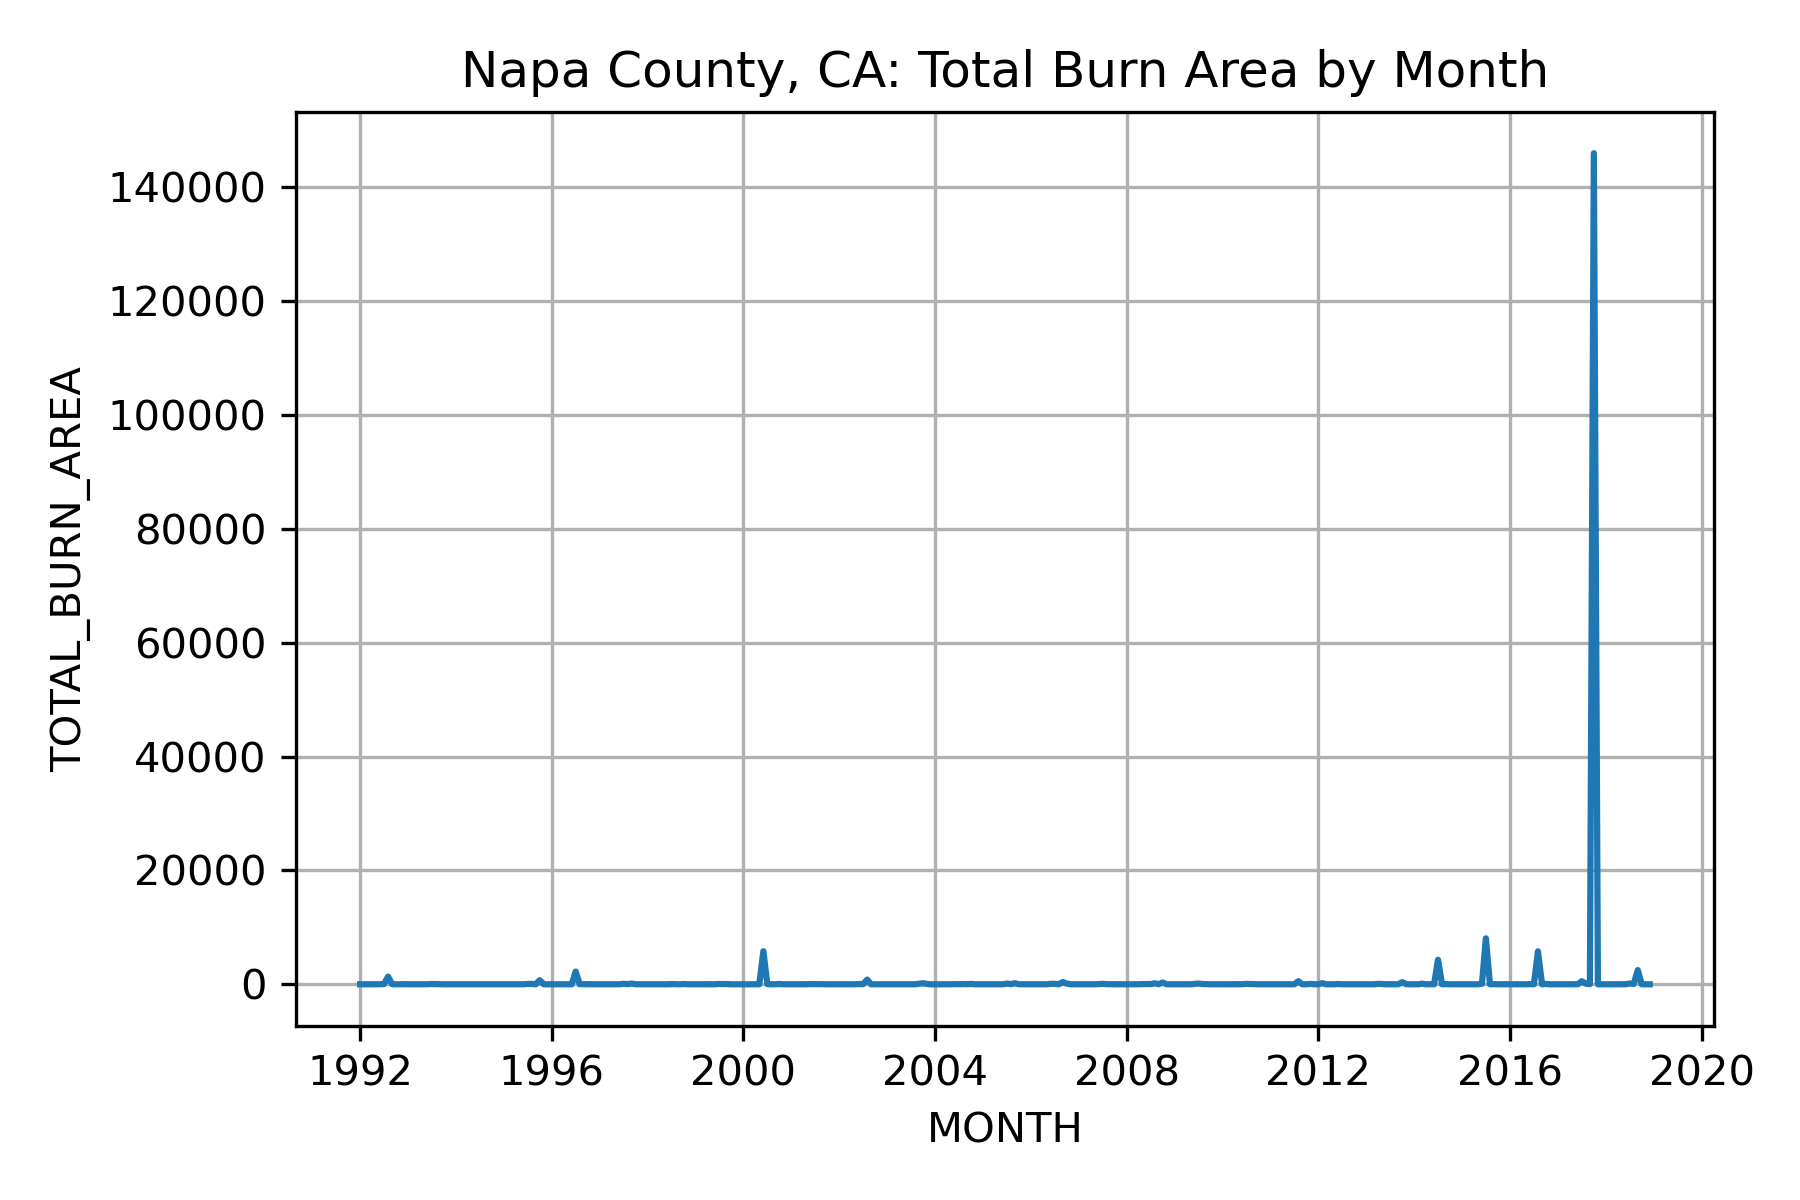
\includegraphics[width=3.5in]{./img/NapaTimeSeriesPlot.png}}

The weather data, which includes temperature and precipitation for the whole state of California is also analyzed with the Napa County data. As expected, weather data is very cyclical on an annual basis with precipitation for California averaging 1.8in per month. The average low temperature for any month is 47.08 degrees Fahrenheit and the average high temperature is 72.49 degrees Fahrenheit. \\[0.3in]

\parpic(3.8in, 2.3in)[l][c]{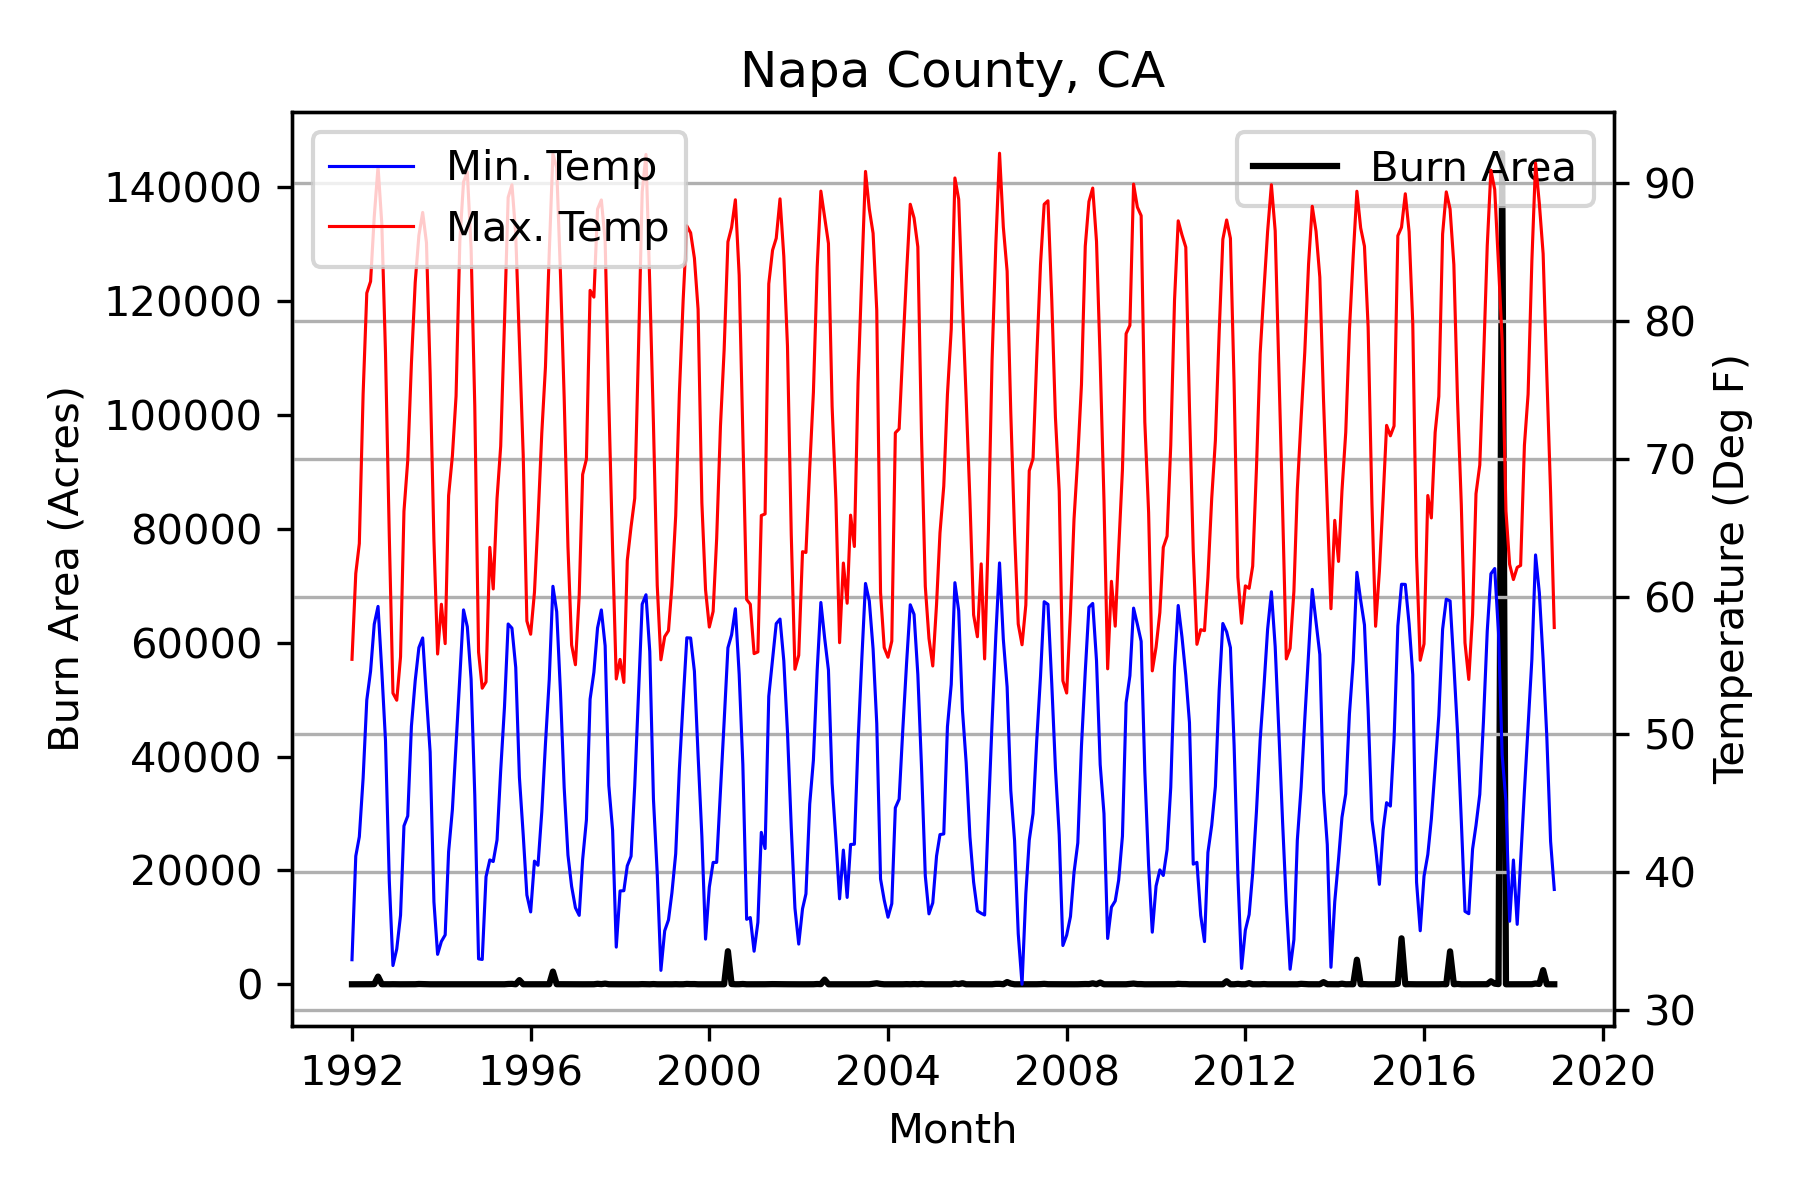
\includegraphics[width=3.65in]{./img/NapaTempPlot.png}}

The variance of the total burn area is very large, with a standard deviation of over 81 thousand. Interestingly enough, when we drop the single maximum from the series the standard deviation drops to 709, indicating that the single largest fire, from 2018, has a major impact on the shape of the data set as a whole. Precipitation is a very stable series with a standard deviation of only 2. Temperature varies slightly more, but is still quite stable. Looking at auto-correlation for Napa County shows no significant auto-correlation for either immediate terms or seasonal lags. This indicates that past values of burn area are not likely to be a good predictor of future burn area. \\

\subsection{\textrm{Elko County, NV}}

Elko County Nevada is an example of more regular, consistently sized fires. The pattern which appears in this series is that roughly every four years, there is a run of larger fires for three years in a row. The plot of the time series shows this trend very distinctly. This pattern also manifests itself in the auto-correlation, from which we can see the the significant correlation in the most recent terms and in the annual lag terms. The average burn area for this county is 12,568 acres which is significantly higher than Napa county, however, the county area for Elko County is 1.101e7 whereas the area of Napa County is 5.045e5. So Elko County is much larger, and therefore it is expected that the average burn area will be so much higher than in Napa County. This underpins the fact that county area is a key variable in the total burn area. \\

\parpic(3.8in, 2.3in)[l][c]{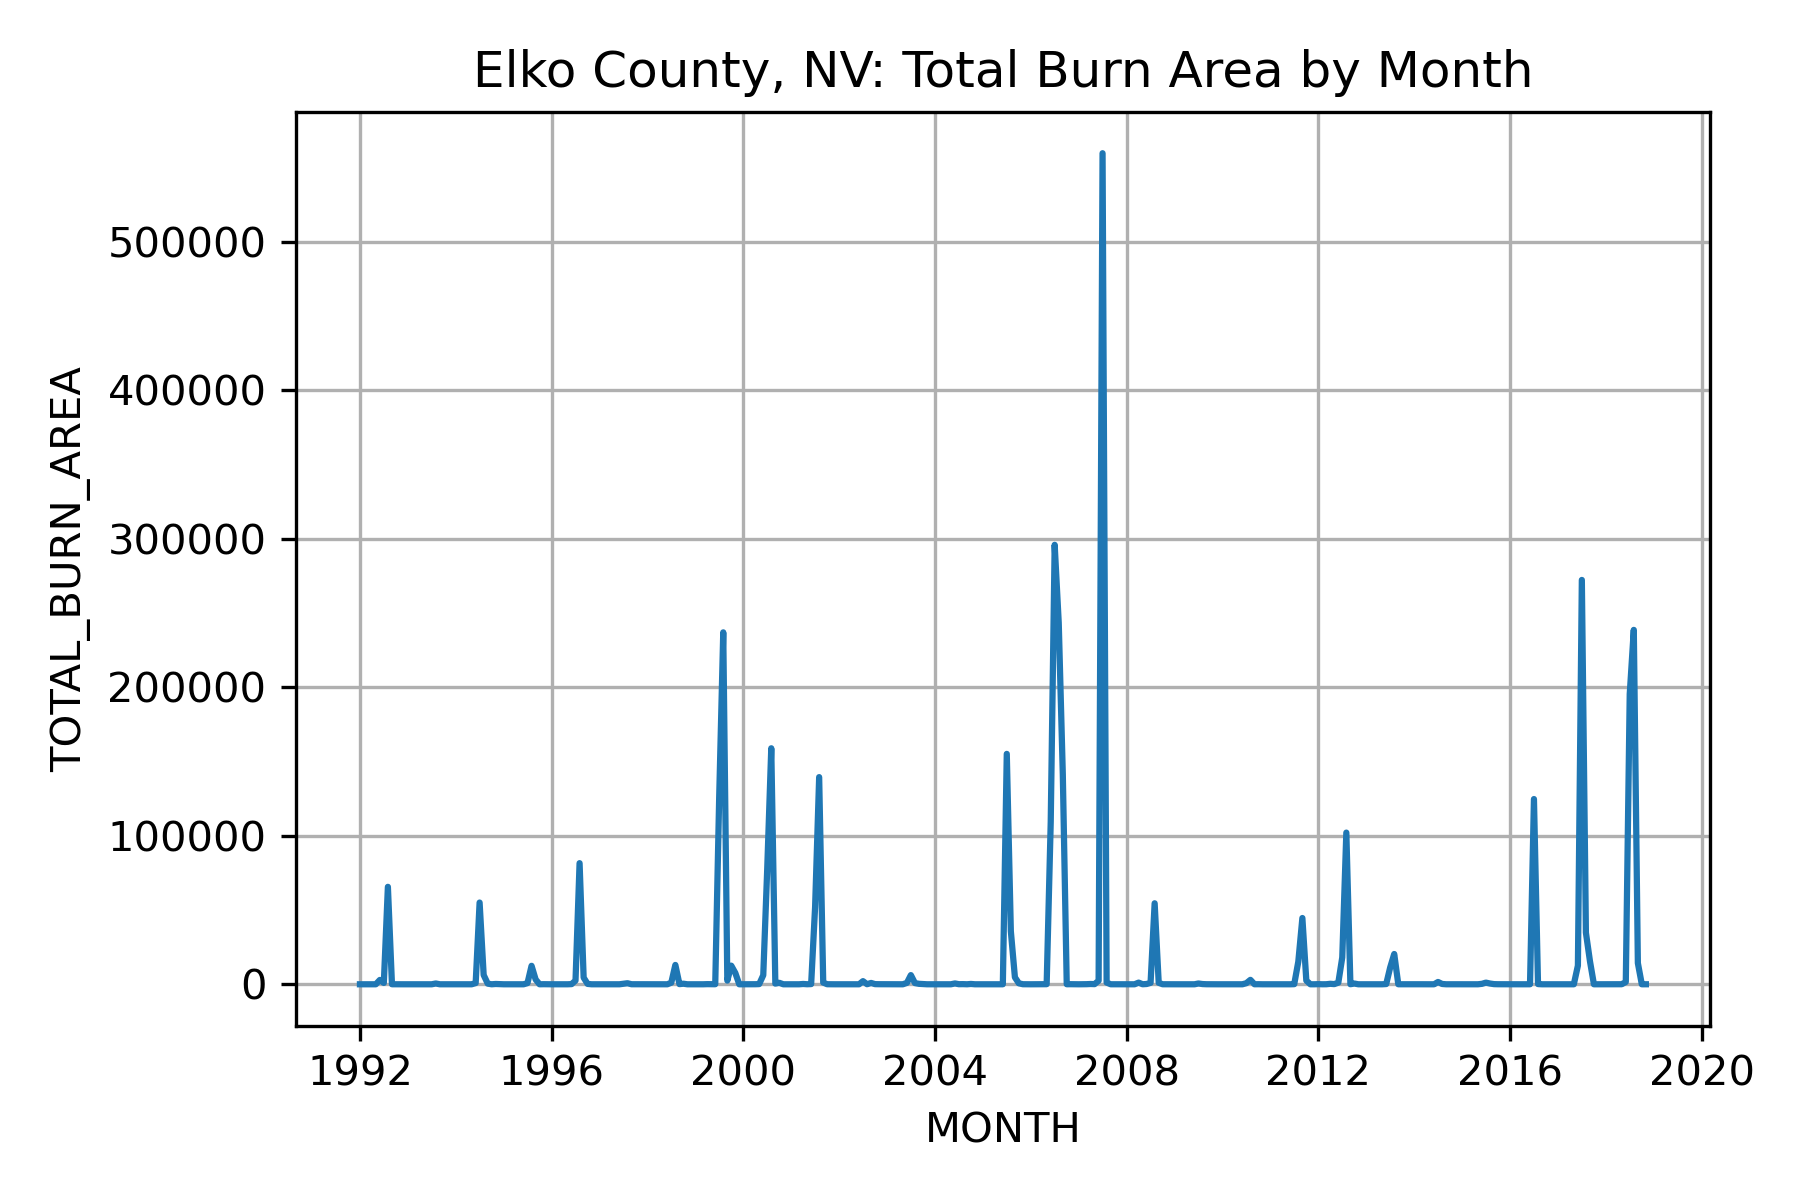
\includegraphics[width=3.65in]{./img/ElkoTimeSeriesPlot.png}}

The precipitation for Nevada is much lower than the precipitation in California, with an average of only 0.7in per month. In addition, the temperature swings are much higher, with an average low temperature of 37 degrees Fahrenheit and an average high temperature of 68 degrees. Also, the average high temperature varies more, with a standard deviation of 16.4 degrees. The min temperature does not vary as much. In practice this indicates to me that the weather is much more volatile in the summer than in the winter, and that there could be a relationship between temperature and variance, which would break any assumptions of stationarity. 

\parpic(3.8in, 2.3in)[r][c]{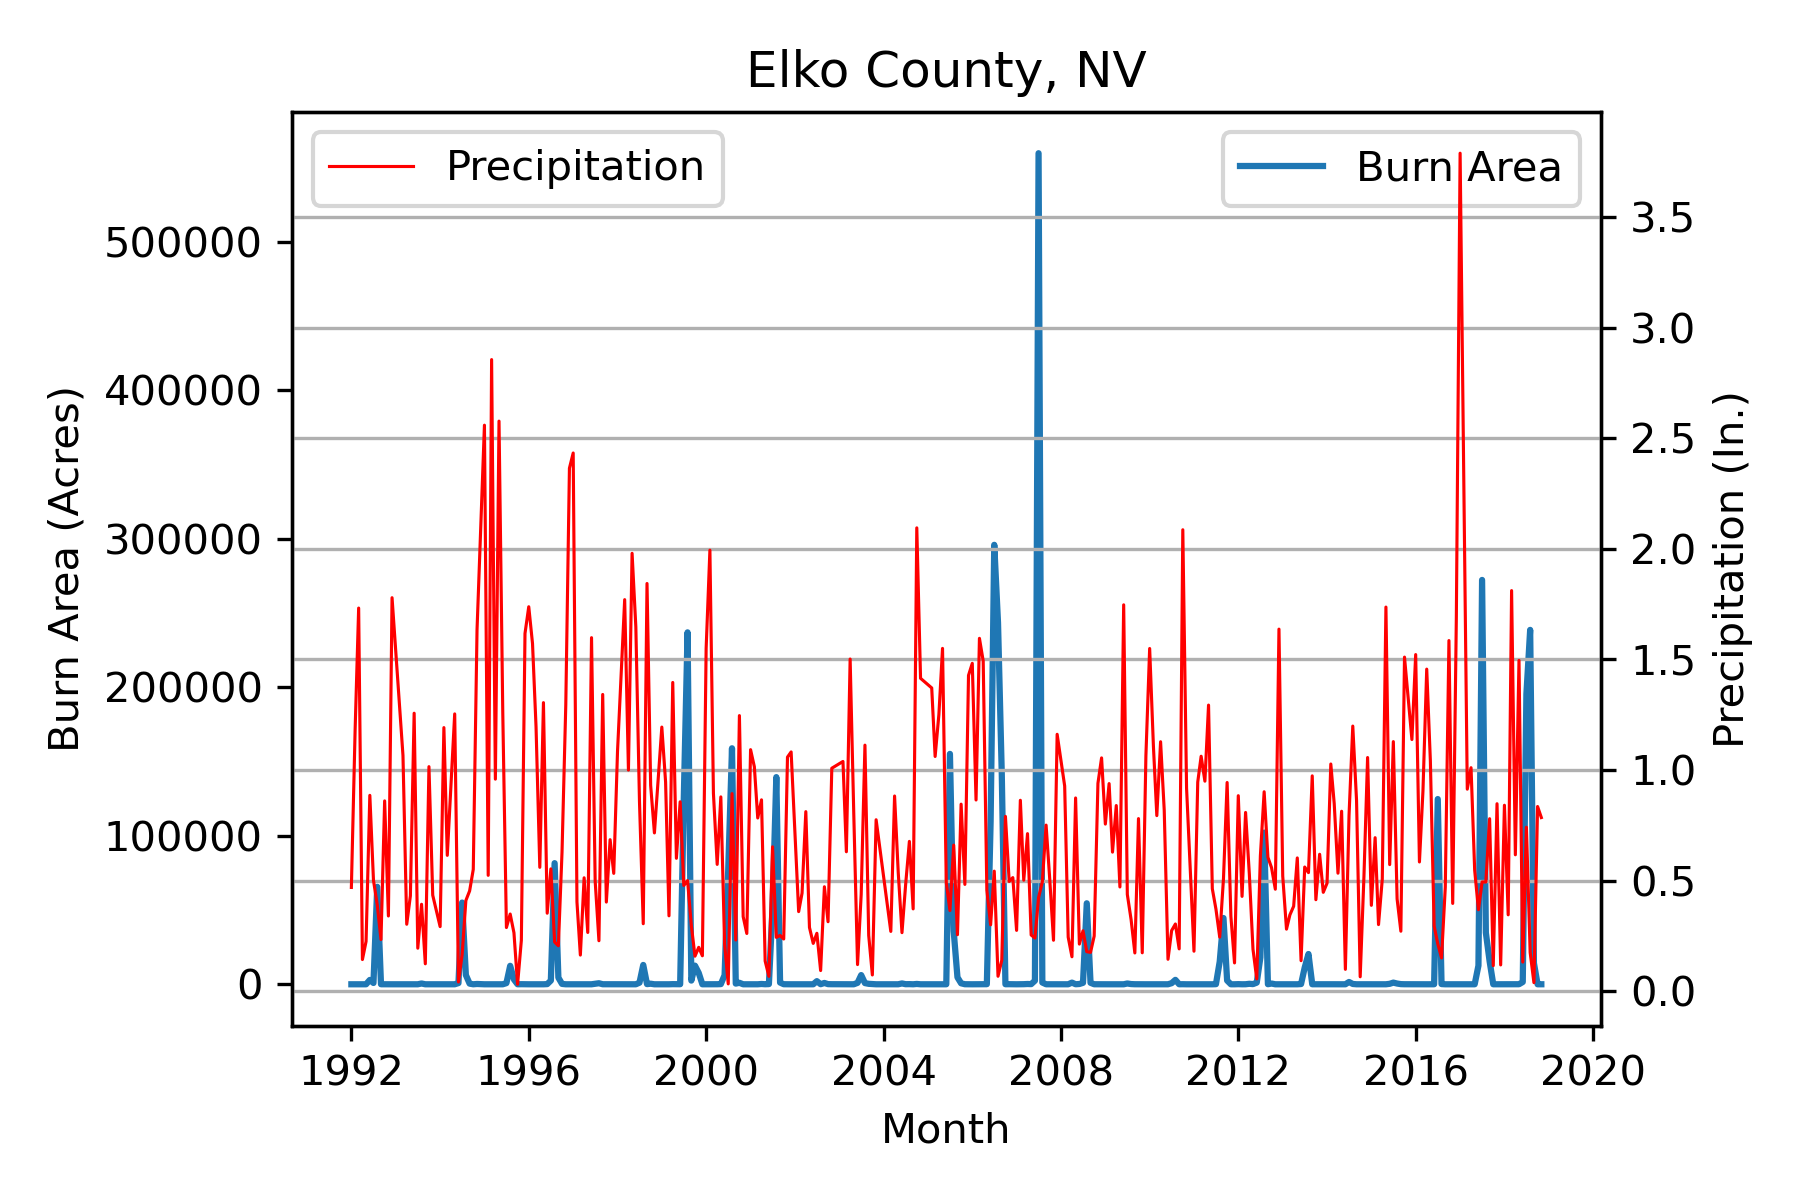
\includegraphics[width=3.65in]{./img/ElkoPrecipPlot.png}}

Discussing the precipitation again. Given that the average precipitation is only 0.7 inches, the standard deviation of 0.56 inches is extremely large. The plot of the precipitation shows that there are very drastic swings in the precipitation levels. These swings could be very highly correlated to the frequency and severity of the fires which are occurring in Nevada. The correlation between precipitation and total burn area is -0.14 which while it is not particularly strong, does align itself with our intuition that when there is less precipitation, and in particular rainfall, there are larger fires. Due to the fact that our weather data is only on a state level, any future analysis may look to obtain weather data on a more granular level, perhaps at the county level itself, if possible. 

\section{\textrm{Modeling}}

We will now discuss the data structure and methodological approach to modeling our data. Give the spatio-temporal structure of our data some compromises had to be made in the formatting of the data. Also, since we don't want to model each county individually, we want to have a systematic way to account for the variations in the counties themselves. Since it is reasonable to believe that something as simple as county level government policy or controlled burn policies could play a major factor in the size of fires. 

\subsection{\textrm{Data Format}}

In preparation of our modeling phase we must make some final preparations to our data. For this project we will use a time-lagged variable approach to our modeling. That is, one of our main input variables is a time-lagged version of the target variable itself. In this way we hope to capture any auto-correlation which may exist between past fires (or the lack thereof) and future fires. We include lags for 1, 2, 3, 4, 5, and 6 periods behind to capture any auto-correlation from immediately prior months. We also include lags of 11, 12, 13, 23, 24, and 25 months to account for any annual auto-correlation which may be due to seasonality in the data. \\

In addition to the time lagged variables of the target variable itself we also time lag our variables for precipitation, and temperature. This allows us to try and model any cumulative effects that may result in larger or smaller fires. Possibly in a scenario where several months in a row with low precipitation would yield a larger fire. For other exogenous variables, such as county area or county itself as a category, since they do not have a temporal relationship we do not create any lagged columns for those variables. 

\subsection{\textrm{Model Framework}} 

Our modeling framework will be based on the decision tree methodology, in particular, using boosted forests of random tree. This methodology is very common in scenarios such as these. Another technique which is common for these types of scenarios is time lagged neural networks (TLNN's), and while TLNN's can yield very good results for these types of problems they are more difficult to construct and tune to achieve the best possible accuracy, so we stick to the simpler, and more easily explainable, decision tree methodology. \\

Our primary algorithm will be a variation of the Extreme Gradient Boosted Random Forests algorithm (XGBoost). This methodology creates random forests, which are comprised of many individual decision trees, and serve as our weak learners for each iteration. Then via the method of gradient descent the new trees are added to the existing forest such that it minimizes a specified loss function. At each iteration, our estimator is fitted and the gradients are updated. In addition to the base algorithm we can introduce sub-sampling which takes only a sub-sample of our data to build each weak learner. There is also a learning rate, which decreases the contribution of an individual regression forest. The learning rate can be thought of as the step length of the gradient descent. The number of iterations, as well as the size and any pruning of the weak learners, as well as, the learning rate are all parameters which must be selected or tuned in some fashion. To select and tune our parameters we will implement a naive grid search approach to help narrow down the best combination of parameters. \\

We now discuss the basic algorithm for Gradient Boosted Forests. We only outline the steps for the boosting, it is a ssumed that we know how to calculate a decision tree model.

\begin{enumerate} \item[1.] Initialize the base model by taking the average of the target column. Then our base model is defined by \begin{equation} F_0(x) = argmin_{\gamma} \sum_{i=1}^{n} L(y_i, \gamma) \end{equation} Where $L$ is our loss function. 

\item[2.] Calculate the psuedo-residual, or the difference between the observed and predicted values. 

\item[3.] Fit a decision tree to the psuedo residuals, call that model $h_m(x)$, where $m$ is the index for the decision tree.

\item[4.] Calculate the output of each leaf by taking the average of all the values in the leaf. The output can be calculated as \begin{equation} \gamma_m = argmin_{\gamma} \sum_{i=1}^{n} L(y_i, F_{m-1}(x_i) + \gamma h_m(x_i)) \end{equation} 

\item[5.] Update the model. For a learning rate $\nu$ the next decision tree is calculated \begin{equation} F_m(x) = F_{m-1}(x) + \nu h_m(x) \end{equation}

\end{enumerate}

To analyze the output of the model we will utilize feature importance which is a concept which quantifies which features are most important based on how often they are used as split points of a tree. We will also use Shapley Additive Explanations to gain additional insights into feature importance. Shapley Additive Explanations is a technique which allows us to "attribute to each feature the change in the expected model prediction when conditioning on that feature" (Citation). Using this game theoretic approach has become very popular as a method for explaining decision tree models in intuitive ways and understanding the impacts that an individual feature has on the overall prediction. \\

The variation which we use for this project allows for better handling of categorical features. The algorithm which we apply here first converts categorical features to one-hot-encoded columns so that we don't have to handle that data transformation before hand. This algorithm is implemented in the Python package CatBoost (reference). 

\subsection{\textrm{Model Fitting}}

Our model is fitted in Python using the package CatBoost. Our first model iteration is fitted with 1000 boosting iterations, we prune our leaves so that each leaf must have at least 10 samples. We also specify that our samples are time dependent so that some of the random shuffling does not take place in the construction of the trees so that the structure is preserved. We also prune our trees so that they only split a maximum of 5 times. Our process for selcting variables is as follows. We first fit a model from only the regression variable, essentially, we remove any variables which are time lags of the target variable itself. From there we use the feature importance to remove un-necessary variables, we set an importance threshold of 0.1. Secondly we add the auto-regressive features, that is, the variables which are lags of the target variable, then we use feature importance to remove any variables, auto-regressive or not, from the resulting model to achieve out final model. We did initial parameter tuning and then retained the same parameters throughout our variable selection.  \\

For determining model accuracy we utilize the root mean squared error, mean absolute percent error and the median absolute error. The reason for the median absolute error is that it is resilient to outliers. The root mean squared error for our second iteration model is 5063 and 12224 for training and testing, respectively. While this metric may show that we have over fitted out model, when we look at the median squared error, which is 118 and 140 for training and testing, respectively, we see that it is likely the effect of some outliers in the testing set which was drastically increasing our RMSE. 

\subsection{\textrm{Model Analysis}}

To analyze our model, we use a Python package called Shap which implements Shapely Additive Explanations to allow us to explain the impacts of different features on our prediction. From the feature importance plot we can determine that the most important features are not exactly what we expected, however, they are relatively intuitive when we think about it. The minimum temperature annual lags which have most impact on our predictions indicate to me that the weather of previous years is important. In general the correlation between temperature and precipitation is quite high so the high importance indicates that weather patterns are important, as a whole. Then we see that we have our first auto-regressive term appearing. From the summary plot we can see that typically higher burn areas for the previous month indicates higher burn areas for the following month, this is logical since if the conditions are ripe for a fire in the previous month, it makes sense that the conditions are once again ripe for a fire in the following month. In practice the relationship between current month burn area and previous burn area likely follows a parabolic shape since if there are little to no fires then the conditions are not likely suited for a fire, however, if there is a very large fire in the previous month then there will likely be little to no fuel for any potential fires to utilize in the current month. It is difficult to tell of the model caught that quadratic relationship or not. \\

\begin{figure}
    \centering
    \subfloat[\centering Feature Importance]{{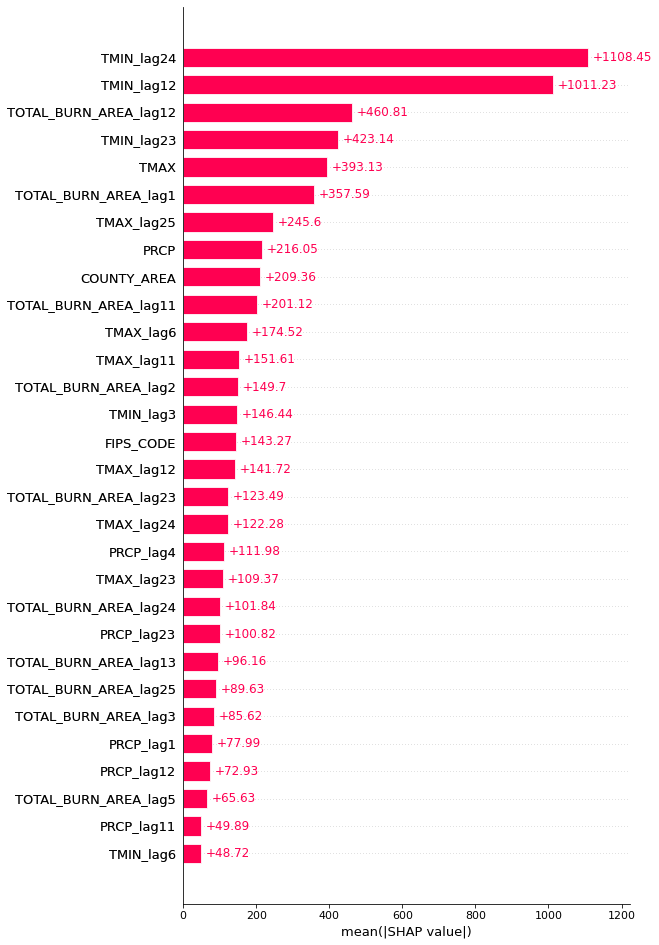
\includegraphics[scale=0.35]{./img/FeatureImportance.png}}}
    \qquad
    \subfloat[\centering Summary Plot]{{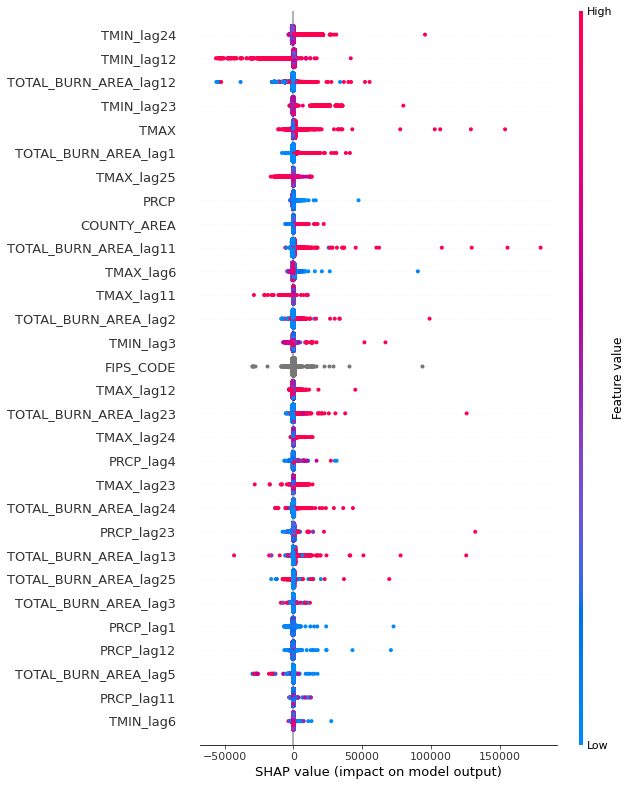
\includegraphics[scale=0.4]{./img/ShapSummaryPlot.png}}}
    \caption{Shap Explainer Plots}
\end{figure}

Another interesting feature which has a lot of importance is the county area, the correlation between burn area for a county and the county area is obvious but the fact that the model placed such high importance on that variable is very promising and indicative of a good model. Also, the general relationship between larger counties and larger burn area is quantified in the summary plot. \\

\parpic(3.8in, 2.3in)[r][c]{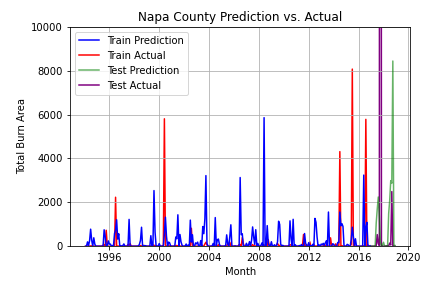
\includegraphics[width=3.65in]{./img/NapaPredPlot.png}}

We return to our example counties to plot some predictions against the actual data for model validation and analysis. Starting with Napa County California we notice that due to the fact that the patterns in the burn area for this county are not evident from any sort of visual analysis. It appears that the spikes are random or at least difficult to determine with any kind of consistency. Indeed, the single large spike from 2018 is a particularly egregious outlier and so ignoring that spike and focusing on the rest of the time frame we can see that while the model predicts lots of small fires, in reality Napa county experiences stretches of no fires at all, with occasional large spikes. It is reasonable to expect that a different model may perform better here, perhaps something which is based on a zero weighted distribution. \\

\parpic(3.8in, 2.3in)[r][c]{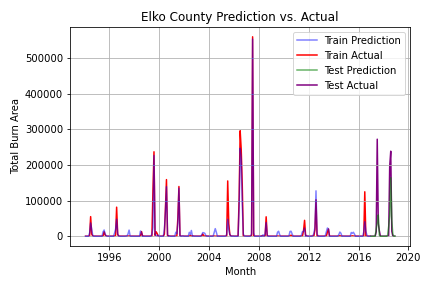
\includegraphics[width=3.65in]{./img/ElkoPredPlot.png}}

Looking at Elko County Nevada we can see that our model performance is much better. For Elko County there are much better defined patterns and consistencies, and our predictions do a good job of maintaining a closeness to the actual patterns. It is also worth noting that Elko county is much larger than Napa county so fires are not likely suppressed, as they would be in a smaller more populous county, such as Napa. That suppression of the wildfires is likely what gives rise to the large spike which we see in Napa County. When, for years and years, no small fires occur, there is a build up of fuel for a prospective fire, so that when a wildfire does occur it becomes much larger than it would have been otherwise. \\


\section{\textrm{Conclusions}}

In conclusion, the data which we are using lends itself well to some simple analysis and modeling to better understand the underlying conditions for wildfires. The analysis and technique demonstrated is a very simple, naive approach to modeling the wildfire data. We were able to fit a model which, most of the time, was able to generate a prediction close to the actual value, when comparing across training and testing sets. Given the spatial-temporal structure of the data there are better modeling alternatives which involve treating the state and county categories as hierarchies in a Hierarchical linear model. Also, time lagged nueral networks have been demonstrated to perform well in these types of scenarios. We opted for the tree based method due to the simplicity and the easy interpretability of the model results. Additional analysis from a Bayesian standpoint may also yield very informative results, where, we can produce a posterior predictive distribution and hence assignt a probability to fires of different sizes occuring, rather than predicting a single point for fire size. This would be particularly valuable for counties such as Napa County California, where the spikes in the data are particularly difficult to handle with a single point prediction. 


\pagebreak

\section*{\textrm{Bibliography}}

\begin{enumerate} 
\item[1.] NWCG (National Wildfire Coordinating Group). 2020. Glossary of wildland fire terminology. Accessed December 2020. www.nwcg.gov/glossary/a-z.


\item[2.] Short, Karen C. 2021. Spatial wildfire occurrence data for the United States, 1992-2018 [FPA\_FOD\_20210617]. 5th Edition. Fort Collins, CO: Forest Service Research Data Archive. https://doi.org/10.2737/RDS-2013-0009.5

\item[3.] Lundberg, Scott M and Lee, Su-In. A Unified Approach to Interpreting Model Predictions. 2017. Advances in Neural Information Processing Systems 30, 4765-4774. http://papers.nips.cc/paper/7062-a-unified-approach-to-interpreting-model-predictions.pdf. 


\end{enumerate}



\end{document}
























